\section{Introduction}

The Morpion Solitaire is a paper-and-pencil single-player game played on a square grid with the initial configuration
  of $36$ dots depicted in Figure~\ref{fig:rules}.
In the 5T variant of the Morpion Solitaire game\footnote{
We refer to this variant as the Morpion 5T game. For an overview of other variants see the webpage \cite{boyer} or the paper \cite{demaine}.}, in each move the player puts a dot on an unused grid position and draws a line that consists of four consecutive segments passing through the dot. 
The line must be horizontal, vertical or diagonal. None of the four segments used in the line may appear as a segment of any other line.  %In the 5T variant of the Morpion Solitaire, the same dot may be used in more than one move of the player and in the 5D variant every dot may be used at most once.  
%In all variants of the Morpion Solitaire 
The goal is to find the longest possible sequence of moves.

%\todo{Do a picture of initial position}
% variables of line 
% 	beginning (two numbers), 
% 	direction 
%		0 - left, 
%       1 left-up, 
%       2 up, 
%       3 right-up, 
%       4 right
%	special point (two numbers)
% 	move number (one number)
% together 6 variables 


\newcounter{curx}
\newcounter{cury}

\newcommand{\unitsize}{0.5cm}
\newcommand{\unitscale}{0.5}

\newcommand*{\linemorpion}[6]{
    \setcounter{curx}{#1}
    \setcounter{cury}{#2}
    \foreach \vertex in {0,...,3}
	{
    	\ifthenelse{\vertex = #5} 
        {
        	\node (current) [draw,circle] at (\value{curx}*\unitscale,\value{cury}*\unitscale) {#6};
        }
        {
        	\node (current) [draw=none] at (\value{curx}*\unitscale,\value{cury}*\unitscale) {};
        }
        \node (new)  at ((\value{curx}*\unitscale+#3*\unitscale,\value{cury}*\unitscale+#4*\unitscale) {};
        \path (current) edge (new); 
        \setcounter{curx}{\value{curx}+#3};
        \setcounter{cury}{\value{cury}+#4};
	}
}

\newcommand*\morpion{
\node(place) at (0,0)  {};
\foreach \edge in {0,...,11}
{ 			
		\ifthenelse{\equal{\intcalcMod{\edge}{2}}{0}} 
        	{ 
				\ifthenelse{\edge < 6}{ 
					\foreach \i in {1,2,3} 
					{
						\node[above of=place] (place) {};
					}
				}
				{	
					\foreach \i in {1,2,3} 
					{
						\node[below of=place] (place) {};
					}
				}
			}
			{
				\ifthenelse{\edge < 8 \AND \edge > 2}
                {
					\foreach \i in {1,2,3}
					{
					\node[right of=place] (place) {};
					}
				}
				{	
					\foreach \i in {1,2,3} 
					{
						\node[left of=place] (place) {};
					}
				}
			}
}
}

\begin{figure}
\begin{center}
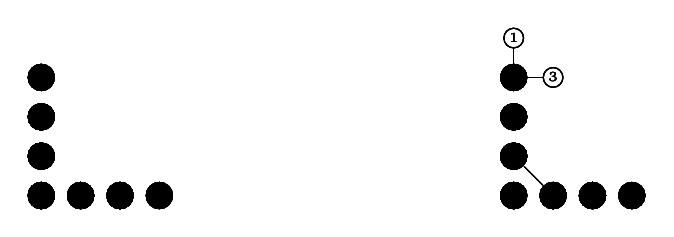
\begin{tikzpicture}%[scale=0.3]
\tikzstyle{every node}=[draw,%
			circle,%
			fill,%
			minimum size  = 0.5*\unitsize,%
			node distance = \unitsize] 
\morpion
\begin{scope}[shift={(6,0)}]
\morpion
\end{scope}
\begin{scope}[shift={(6,0)}]
\tikzstyle{every node}=[minimum size  = 0.5*\unitsize,%
			node distance = unitsize,{font=\tiny},inner sep=0pt] 
\linemorpion{0}{4}{0}{-1}{0}{1}
\linemorpion{1}{0}{-1}{1}{2}{2}
\linemorpion{1}{3}{-1}{0}{0}{3}
\end{scope}
\end{tikzpicture}
\caption{Initial position of Morption 5T on the left and a position with 3 moves on the right.}
\label{fig:rules}
\end{center}
\end{figure}




The problem is notoriously difficult for computers. 
For $34$ years, in the Morpion 5T game the longest known sequence was one of $170$ moves discovered by C.-H. Bruneau in $1976$ (see\footnote{Regarding this and other records we refer to the webpage \cite{boyer} for a detailed description and further references.} \cite{boyer}). % \cite{boyer} the webpage \cite{boyer} provides more details about this record).
%Until $2010$, the record for a computer-generated sequence was $146$ moves, obtained by H. Akiyama, obtained using a Monte Carlo type algorithm.
The record was finally broken by Christopher D. Rosin, who presented in \cite{rosin} a configuration of $177$ moves, obtained using a Monte Carlo algorithm called Nested Rollout Policy Adaptation (NRPA). 
In $2011$ (see \cite{boyer}) he improved his record to $178$, which is the best result known today.
The webpage \cite{boyer} maintained by Christian Boyer, contains an extensive and up-to-date information about records in all Morpion Solitaire variants.

As the Morpion 5T game is played on a potentially infinite grid, a priori it is not clear whether the maximal sequence should be finite at all. 
An upper bound of $705$ was shown in~\cite{demaine}.
In the present paper we show a new upper bound of~$485$. We base our approach on the observation that a Morpion 5T game may be expressed as a mixed-integer linear programming problem.

We observed (see Section \ref{inf_grid}) that the bound obtained by a continuous-valued linear relaxation of the Morpion 5T game significantly depends on the size of the grid on which the game is played. On big grids the bound may be well over the upper bound of $705$ (in fact, we do not know if it is finite). On the other hand on smaller grids we obtained useful bounds. For example, on a grid limited to a regular octagon\footnote{This is a graph that plays a role in the proof of the $705$ bound in~\cite{demaine}.} with sides of length $10$, we obtain a linear relaxation bound of $543$.
By a geometric reasoning, using the notion of potential and careful analysis of the rules of Morpion 5T game, we show that every Morpion 5T position must be contained in one of \theoctagons octagonal grids with small boundaries (see Lemma \ref{lem:octagons} for a precise formula). The maximum bound of $586.82$ is obtained on a grid which is an octagon with sides of lengths $10,8,10,12,10,8,10,12$ (see Figure \ref{therecord}).

In fact, the picture is more complicated. To state a linear problem for Morpion 5T we need not only to consider the shape of the octagonal grid but also a position of the initial cross inside. This makes the number of cases to consider larger by two orders of magnitude. To get around this difficulty we consider variants of Morpion Solitaire called Morpion 5T+ and Morpion 5T++ (see \cite{boyer}). In the later variant the position of the initial cross inside of the grid is not relevant.
%There are two variants of interest here called . 
Every Morpion 5T game is also a Morpion 5T+ game and every Morpion 5T+ game is a Morpion 5T++ game.
The difference between 5T and 5T+ is that the line drawn in a move needs not to pass through the dot placed in this move.
The difference between 5T+ and 5T++ is that one may place more than one dot in a single move, as long as in the final position the number of dots is equal to the number of moves plus $36$. That is, we may borrow dots in 5T++ as long as the balance at the end is correct. In Morpion 5T++ we start with an empty board.

The upper bound of $705$ moves proved in \cite{demaine} is also valid in the Morpion 5T++ game. The longest known sequence of moves in Morpion 5T+ was found by Marc Bertin in $1974$ and consists of $216$ moves (see \cite{boyer}). The longest known sequence of moves in the Morpion 5T++ game was found by Christian Boyer in $2011$ (see \cite{boyer}). The sequence consists of $317$ moves. 

%We observed that the difference between optimal solutions of continuous-valued linear relaxations of 5T, 5T+ and 5T++ is very small. 
The associated mixed-integer linear problems are much easier to solve in the case of 5T++ variant and we have a benefit of much smaller number of cases to consider. However, the limit on the size of the grid pertains to the 5T variant, so our new upper bound of $485$ is valid for the 5T variant only.

The paper is organized as follows. In Section \ref{linear} we formulate the linear problem (\ref{lp0})---(\ref{lp3}). In Section \ref{board_bound} we calculate that the number of instances, which must be treated by the solver, is \theoctagons. In Section \ref{linear_bound} we consider consequences of the relaxation of the original problem (\ref{lp0})---(\ref{lp3}). This allows to show an upper bound of $586$ moves in the Morpion 5T game. In Section \ref{mip_bound} we push the result of Section \ref{linear_bound} in order to obtain an upper bound of $485$ moves. This is done at a considerable increase in the computation time. In Section \ref{geometry} we explain the correctness of algorithms used in previous Sections. The correctness result boils down to an observation how, in terms of potential, a given board relates to the smallest octagon containing this board (see Theorem \ref{thm:octagonalization}). 

We note that modern LP solvers have no problem in finding the record sequence of $317$ moves for the 5T++ variant, but despite considerable computational effort we were not able to break this record. %\footnote{An unfinished computation, terminated after $126$ days, proved an upper bound of $421$ on the octagonal board with edges of lengths $10, 8, 10, 12, 10, 8, 10, 12$.}. 
The current upper bound of $485$ can be improved with more computational resources. However, we believe that the best approach would be to find better limitations on the size of grids. %It is relatively easy to prove that the sequence of $317$ moves is optimal for Morpion 5T++ on smaller (but not very small) grids. We also proved that $317$ is optimal on 10, 8, 10, 12, 10, 8, 10, 12 grid under an additional constraint that the solution is center-symmetric.

It is also possible to write linear programs that solve the Morpion 5D variant of the Morpion Solitaire (see \cite{boyer} for description of the rules and current lower and upper bounds). On larger grids we obtain objective $144$ for the relaxed problem, as the standard potential-based argument applies to the relaxed case as well (see\footnote{In fact, applying additional argumentation, in \cite{demaine} is shown a bound of $141$ moves.} \cite{demaine}). The upper bound of 121 moves in the Morpion 5D game was proved in \cite{japonczycy}. Using variants of the Morpion 5D game and a different strategy of limiting grids, we were able to prove that an upper bound in the Morpion 5D game is below $100$. We also proved that the best possible result in the symmetric Morpion 5D game is $68$. These results will be presented in a separate publication. % will be subject of another report.
